\documentclass[11pt]{article}
\usepackage[utf8]{inputenc}
\usepackage[spanish]{babel}
\decimalpoint
\usepackage{amsmath}
\usepackage{amsthm}
\usepackage{amssymb}
\usepackage{graphicx}
\usepackage[margin=0.8in]{geometry}
\usepackage{fancyhdr}
\usepackage[inline]{enumitem}
\usepackage{float}
\usepackage{cancel}
\usepackage{bigints}
\usepackage{listings}
\usepackage{xcolor}
\usepackage{listingsutf8}
\usepackage{algpseudocode}
\usepackage{algorithm}
\usepackage{apacite}
\usepackage{tcolorbox}
\usepackage{multicol}
\usepackage{tipa}
\usepackage{caption} 
\pagestyle{fancy}
\usepackage{hyperref}
\usepackage{mathtools}% http://ctan.org/pkg/mathtools

\hypersetup{
    colorlinks,
    citecolor=black,
    filecolor=black,
    linkcolor=black,
    urlcolor=black
}
\newcommand{\xvdash}[1]{%
	\vdash^{\mkern-10mu\scriptscriptstyle\rule[-.9ex]{0pt}{0pt}#1}%
}
\setlength{\headheight}{15pt} 
\lhead{Tarea 2. Implementación de un token-ring}
\rhead{\thepage}
\lfoot{ESCOM-IPN}
\renewcommand{\footrulewidth}{0.5pt}
\setlength{\parskip}{0.5em}
\newcommand{\ve}[1]{\overrightarrow{#1}}
\newcommand{\abs}[1]{\left\lvert #1 \right\lvert}
\newcommand{\blank}{\text{\textcrb}}
\date{\today}
\title{Tarea 2. Implementación de un token-ring}
\author{Sanchez Mendez Edmundo Josue}

\lstdefinestyle{customc}{
	belowcaptionskip=1\baselineskip,
	breaklines=true,
	frame=L,
	xleftmargin=\parindent,
	language=C++,
	showstringspaces=false,
	basicstyle=\ttfamily,
	keywordstyle=\bfseries\color{green!40!black},
	commentstyle=\itshape\color{purple!40!black},
	identifierstyle=\color{blue},
	numbers=left,
	stringstyle=\color{orange},
}

\lstset{escapechar=@,style=customc,tabsize=3,language=C++}

\bibliographystyle{apacite}
\begin{document}
		\begin{titlepage}
			\begin{center}
				
				% Upper part of the page. The '~' is needed because \\
				% only works if a paragraph has started.
				
				\noindent
				\begin{minipage}{0.5\textwidth}
					\begin{flushleft} \large
						
\includegraphics[width=0.5\textwidth]{resources/ipn.png}
					\end{flushleft}
				\end{minipage}%
				\begin{minipage}{0.55\textwidth}
					\begin{flushright} \large
						
\includegraphics[width=0.5\textwidth]{resources/escom.png}
					\end{flushright}
				\end{minipage}
				
				\textsc{\LARGE Instituto Politécnico Nacional}\\[0.5cm]
				
				\textsc{\Large Escuela Superior de Cómputo}\\[1cm]
				
				% Title
				
				{ \huge Tarea 2. Implementación de un token-ring  \\[1cm] }
				
				{ \Large Unidad de aprendizaje: Desarrollo de Sistemas Distribuidos} \\[1cm]
				
				{ \Large Grupo: 4CV11 } \\[1cm]
				
				\noindent
				\begin{minipage}{0.5\textwidth}
					\begin{flushleft} \large
						\emph{Alumno:} \\
						Sanchez Mendez Edmundo Josue
					\end{flushleft}
				\end{minipage}%
				\begin{minipage}{0.5\textwidth}
					\begin{flushright} \large
						\emph{Profesor:} \\
						Pineda Guerrero Carlos 
					\end{flushright}
				\end{minipage}
				
				\vfill
				% Bottom of the page
				{\large {\today}}
			\end{center}
		\end{titlepage}
	
	\titlepage
	\tableofcontents
	\newpage
	
	\section{Introducción}
		Mediante el desarrollo de un sistema distribuido el cual tendrá una topología lógica de anillo en donde interceden 4 nodos y la comunicación sera por medio de sockets seguros, sera transmitido un token el cual pasara por toda la topología e ira aumentando de valor en 1, el token será un número entero de 64 bits.\par	
		El funcionamiento del programa es el siguiente:
		\begin{enumerate}
			\item Al principio el nodo 0 enviará el token al nodo 1.
			\item El nodo 1 recibirá el token y lo enviará al nodo 2.
			\item El nodo 2 recibirá el token y lo enviará al nodo 3.
			\item El nodo 3 recibirá el token y lo enviará al nodo 0.
			\item El nodo 0 recibirá el token y lo enviará al nodo 1.
			\item Ir al paso 2.
		\end{enumerate}
	\section{Desarrollo}
Una vez programado el sistema distribuido con base en los algoritmos establecidos en la tarea se procedió a implementar los sockets seguros, para lo cual fue necesario la creación de los keystore tanto para el cliente como para el servidor, la creación del keystore para el servidor la podemos ver en la figura 1 y la creación del keystore para el cliente la podemos ver en la figura 2.
		\begin{figure}[H]
			\centering
			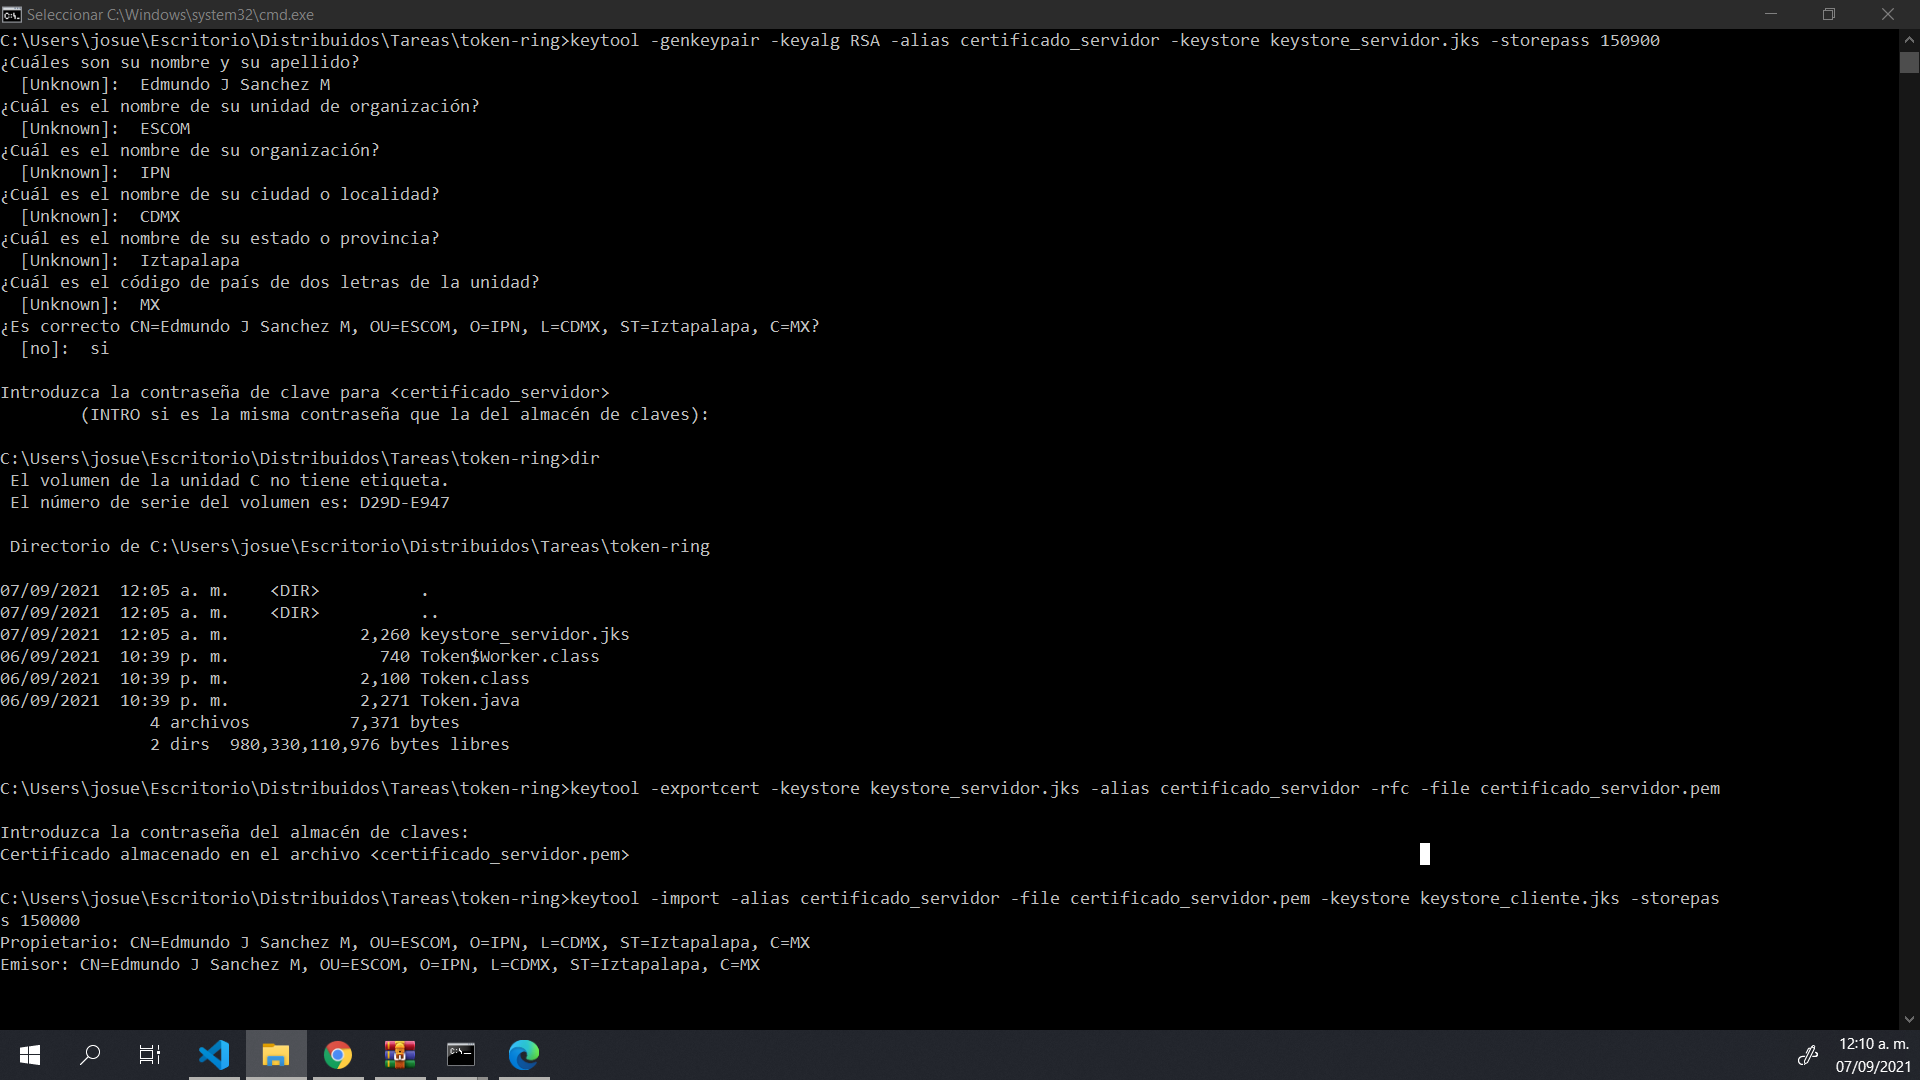
\includegraphics[scale=0.34]{resources/certificado_servidor.png}
			\caption{Creación del keystore para el servidor. }\label{fig:picture}
		\end{figure}
		\begin{figure}[H]
			\centering
			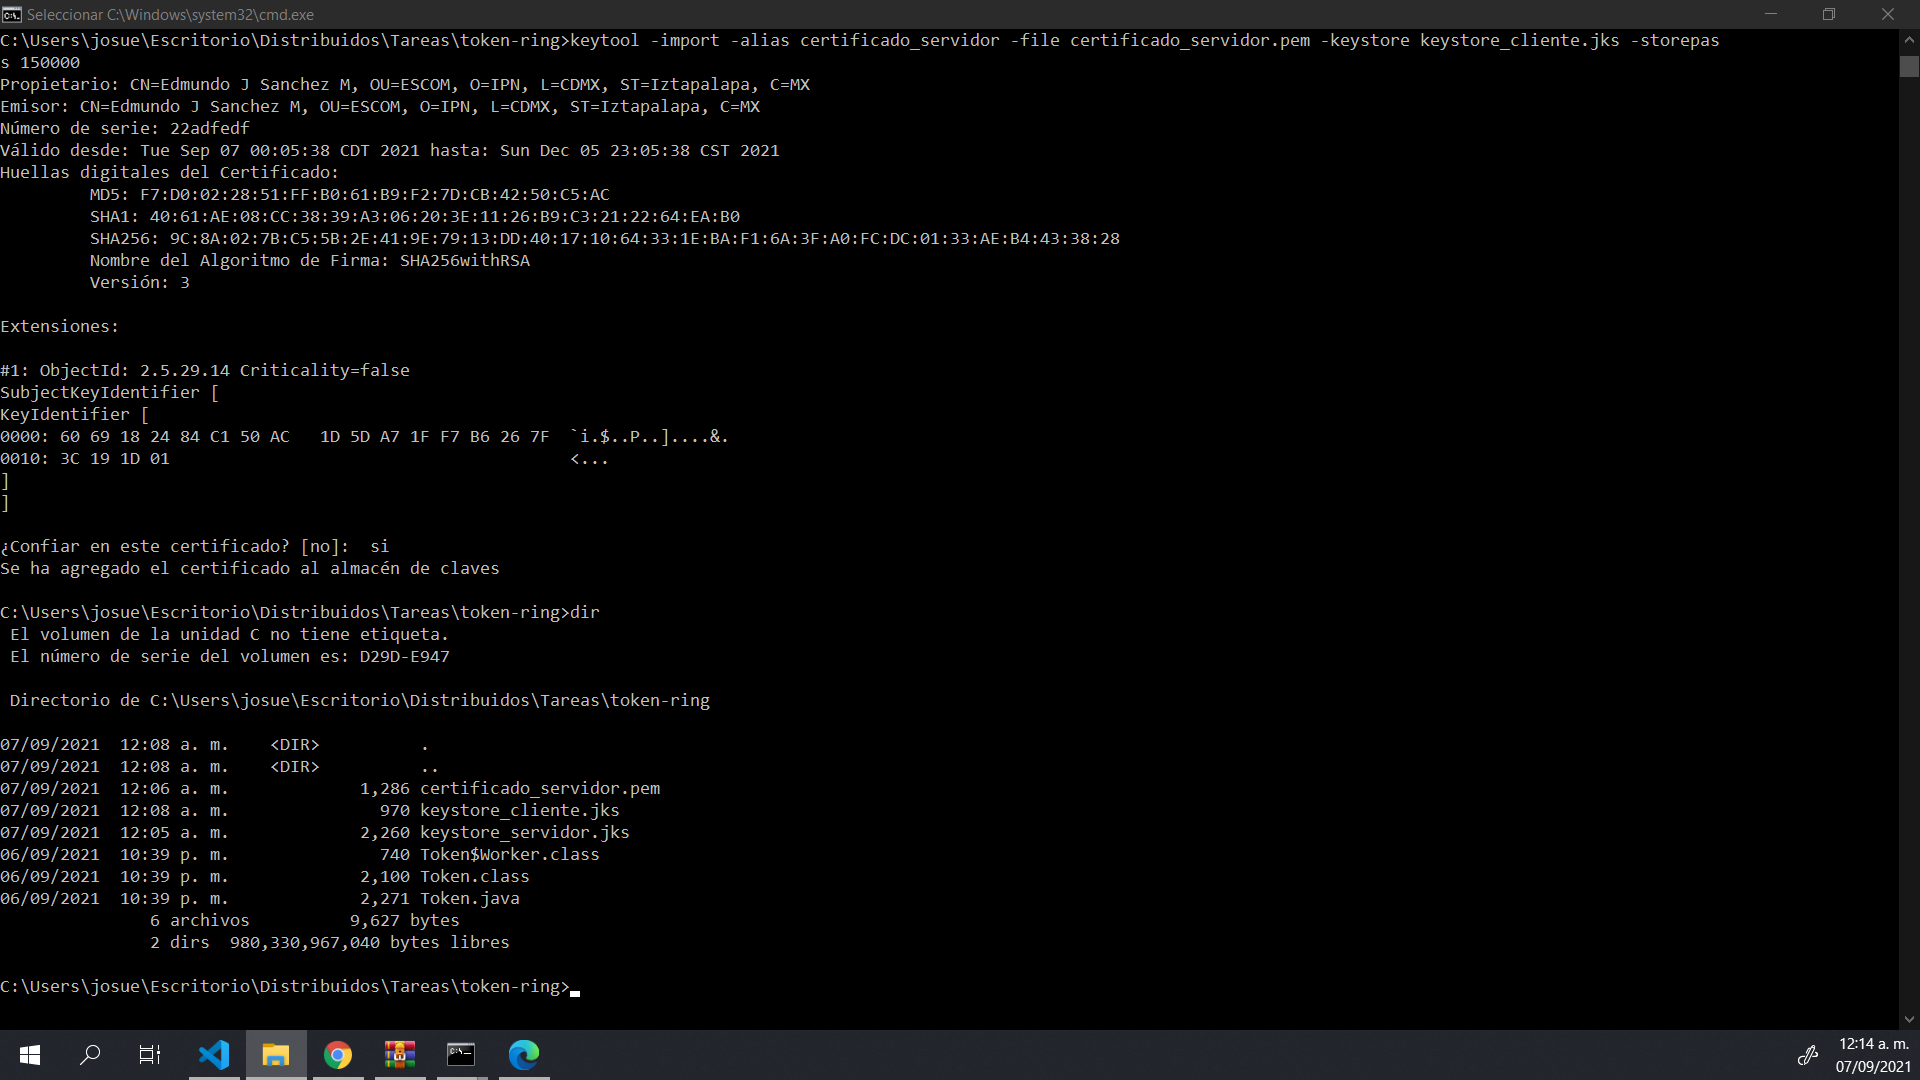
\includegraphics[scale=0.34]{resources/certificado_cliente.png}
			\caption{Creación del keystore para el cliente. }\label{fig:picture}
		\end{figure}
Una vez creado los keystore se procede a implementar lo sockets, empezamos a colocar propiedades del sistema los cuales contienen los archivos con las keystore del cliente y del servidor y las contraseñas correspondientes, todo lo anterior en las lineas 40-43, después en la linea 49 creamos la variable cliente de tipo SSLSocketFactory y asignar lo siguiente (SSLSocketFactory) SSLSocketFactory.getDefault()$;$ para después remplazar el paso 5.1.1 y asignar a la variable conexion la siguiente linea de código cliente.createSocket(ip, 20000 + (nodo + 1) \% 4)$;$ lo cual nos permite crear un socket seguro para el cliente, después para nuestro servidor al inicio del algoritmo 1 justo después crear el bloque try declaramos la variable socket\_ factory de tipo SSLServerSocketFactory y asignamos el valor siguiente (SSLServerSocketFactory) SSLServerSocketFactory.getDefault()$;$ para después remplazar el punto 1.2 del algoritmo 1 y signar a la variable servidor lo siguiente socket\_ factory.createServerSocket(20000 + nodo)$;$\par
Para finalizar se debe si o si cerrar la variable salida, entrada y conexion para que no se tenga error alguno, esto se tendrá que hacer justo después del ciclo del paso 8 del algoritmo 2. 
		\subsection{Compilación del código}
		En la figura 3 podemos ver como la compilación de nuestro programa Token.java se hace de manera exitosa y sin ningún error alguno, esto desde el Símbolo del sistema (CMD) de Windows 10.
		\begin{figure}[H]
			\centering
			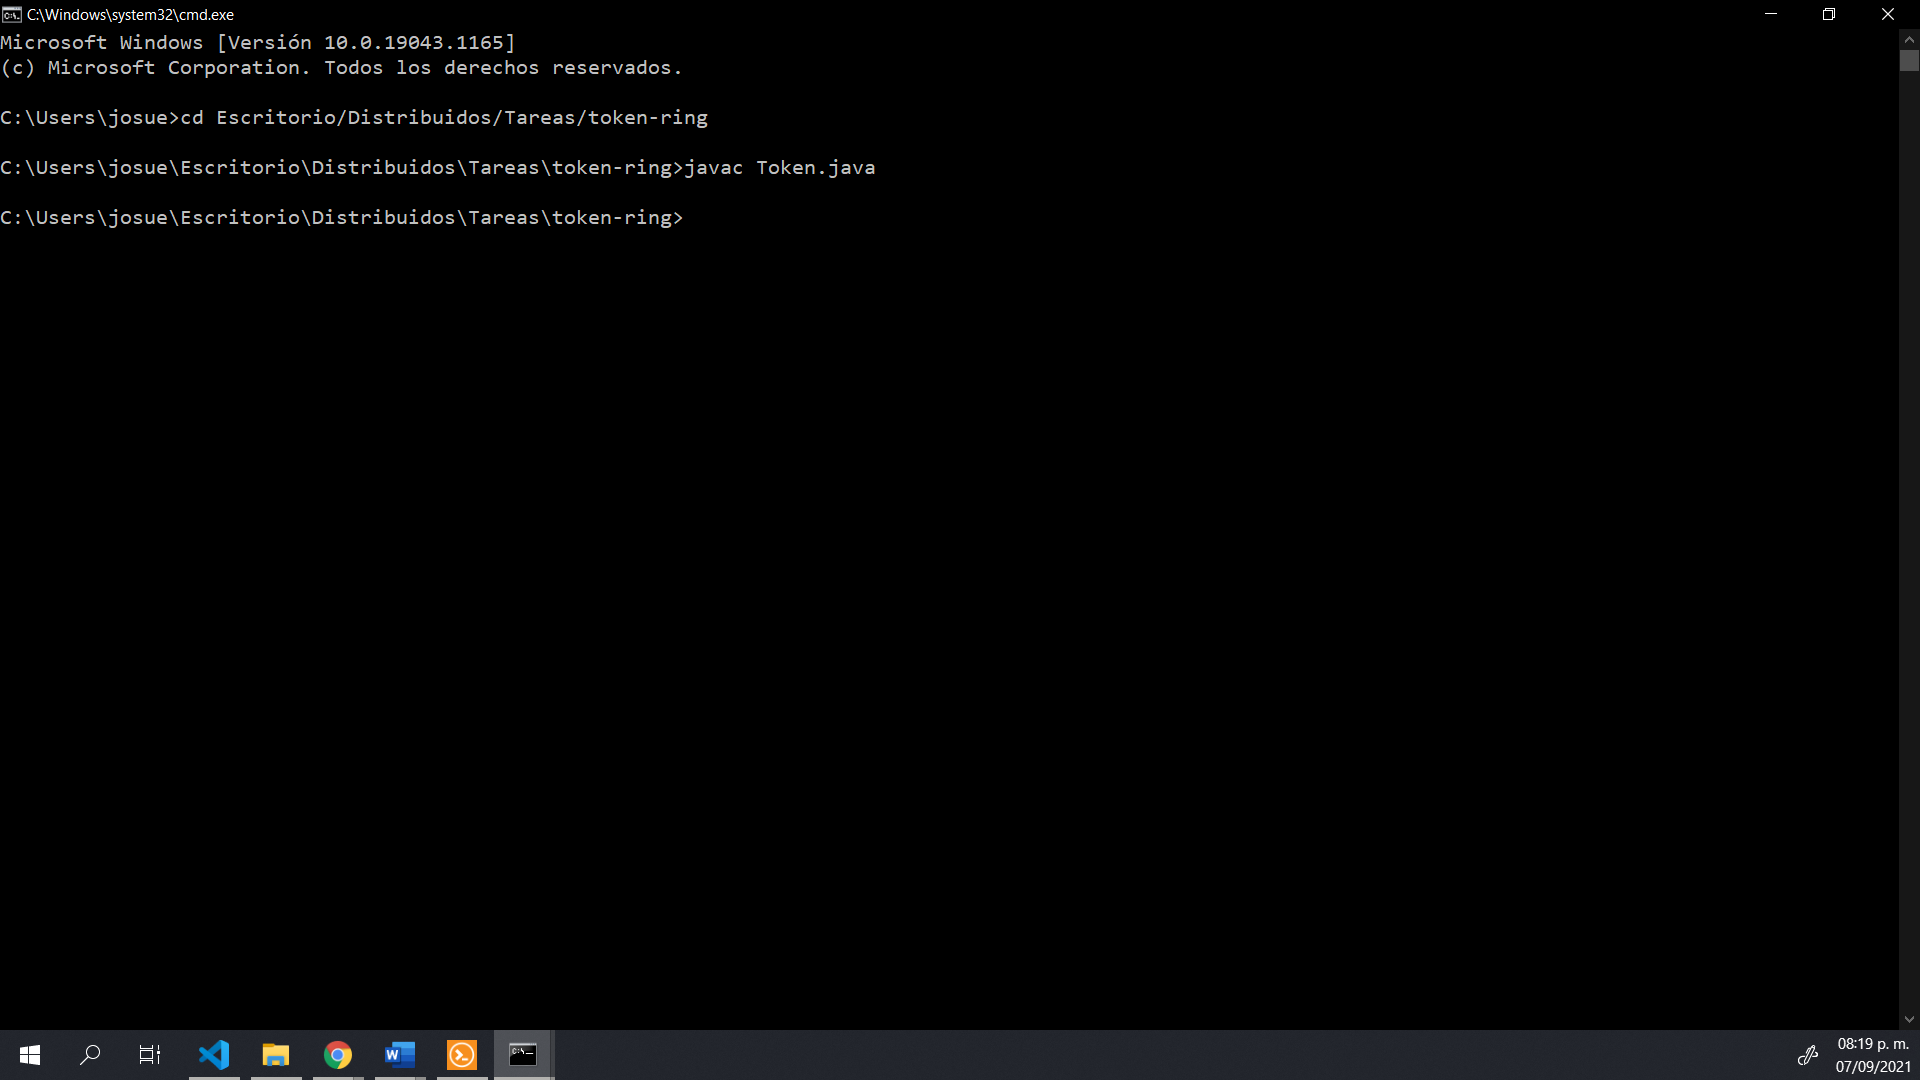
\includegraphics[scale=0.34]{resources/compilacion.png}
			\caption{Compilación del código por medio de CMD. }\label{fig:picture}
		\end{figure}
		\subsection{Ejecución del programa}
		Una vez compilado se ejecuta nuestro programa para lo cual necesitamos abrir 4 consolas y ejecutar los nodos 0, 1, 2, 3 para cumplir con el sistema distribuido, en la figura 4 podemos ver el inicio de estas 4 consolas al ejecutar el programa:
		\begin{figure}[H]
			\centering
			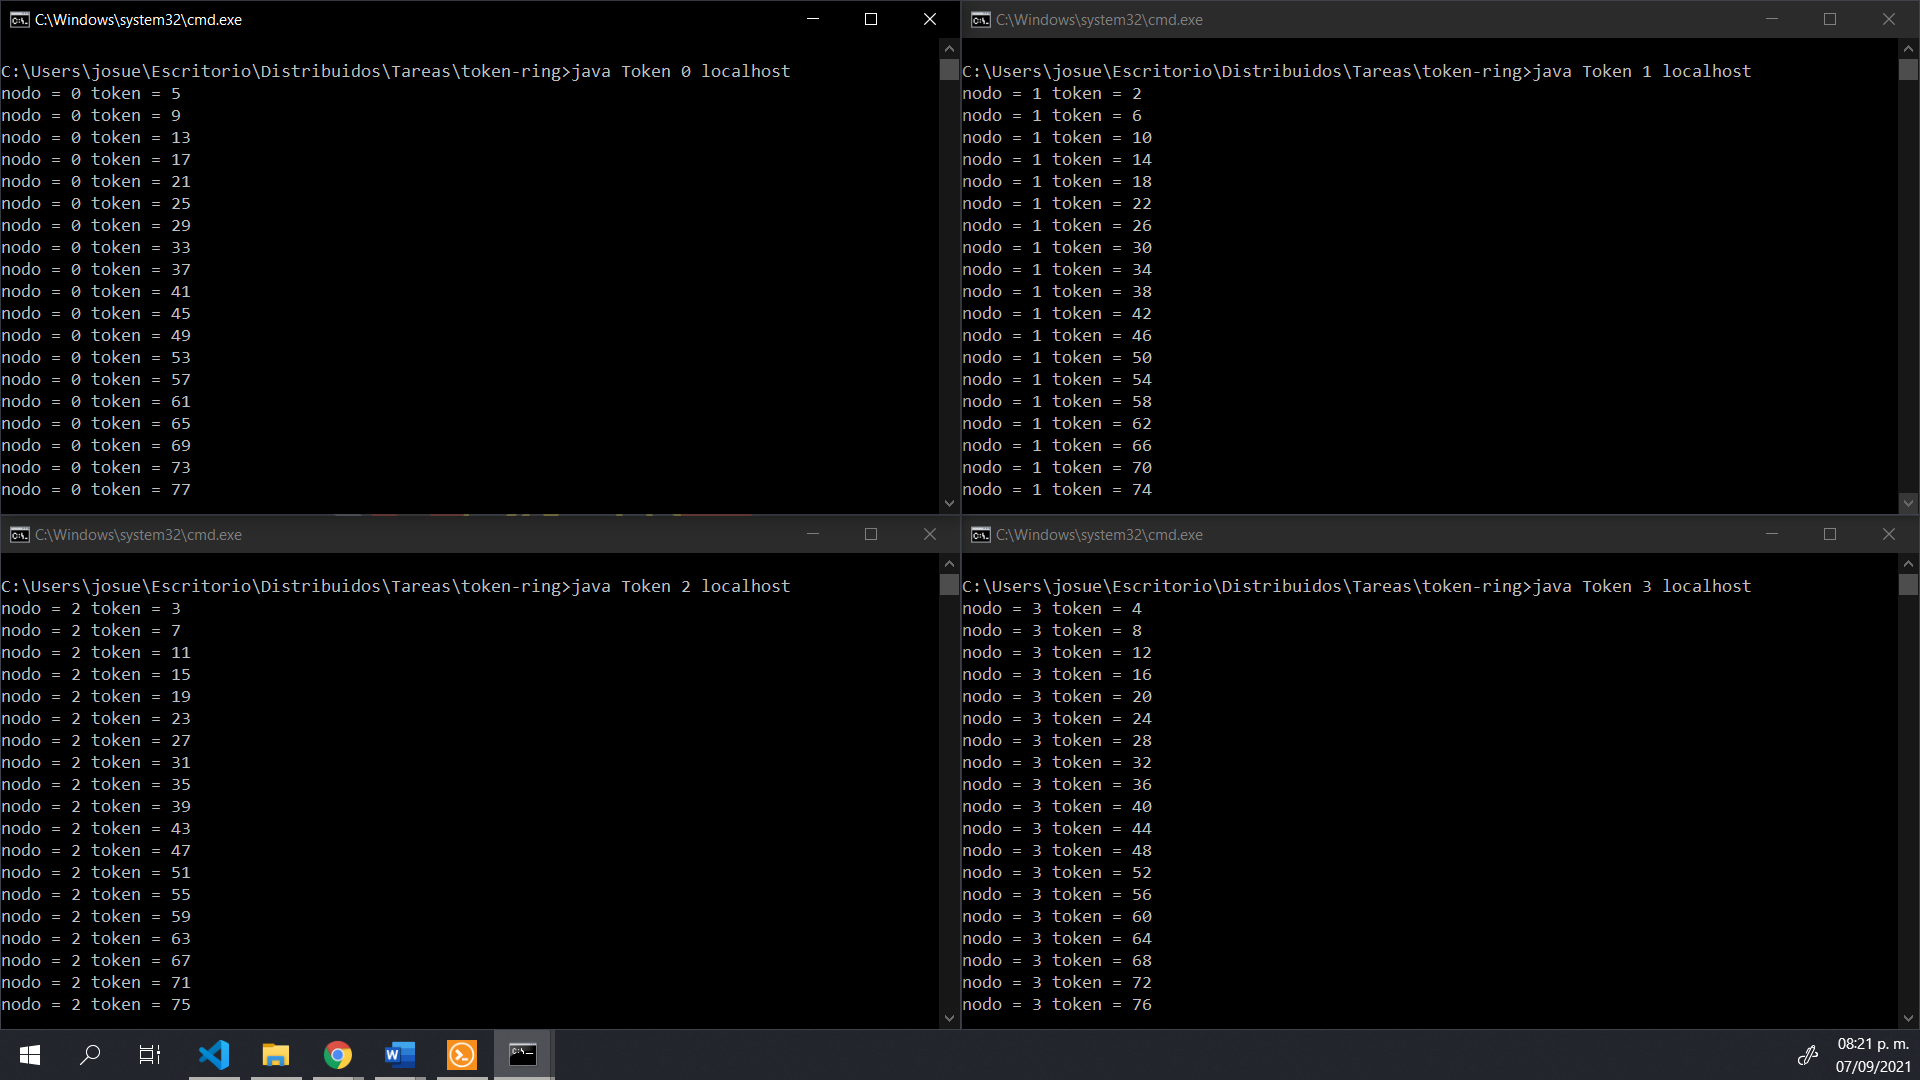
\includegraphics[scale=0.34]{resources/ejecucioninicio.png}
			\caption{Consolas justo después de ejecutar el programa. }\label{fig:picture}
		\end{figure}
		Al finalizar se nos muestra lo que podemos ver en las figuras 5 y 6, se decidió tomar una screenshot mas para visualizar de una mejor manera el resultado de los nodos 2 y 3:
		\begin{figure}[H]
			\centering
			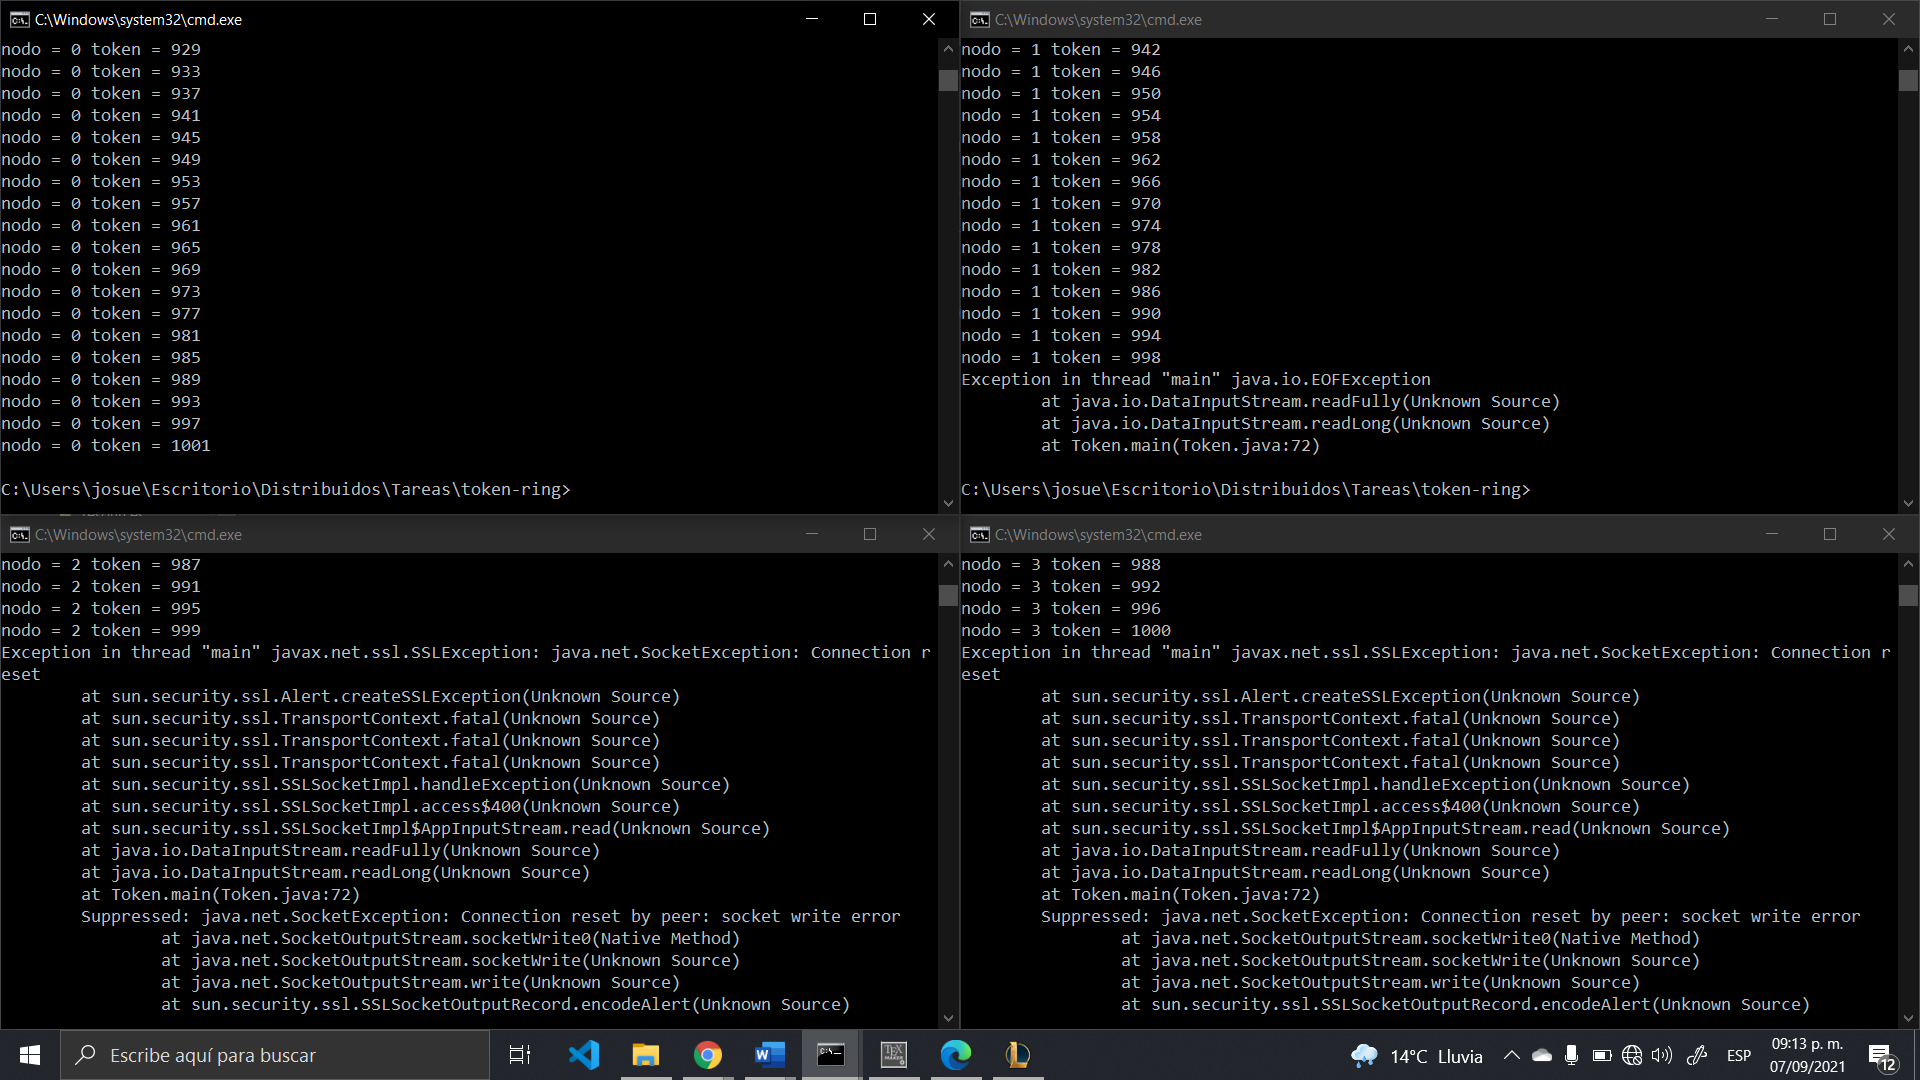
\includegraphics[scale=0.42]{resources/ejecucionfin0.png}
			\caption{Consolas un poco antes del fin de lo ejecución del programa.}\label{fig:picture}
		\end{figure}
		\begin{figure}[H]
			\centering
			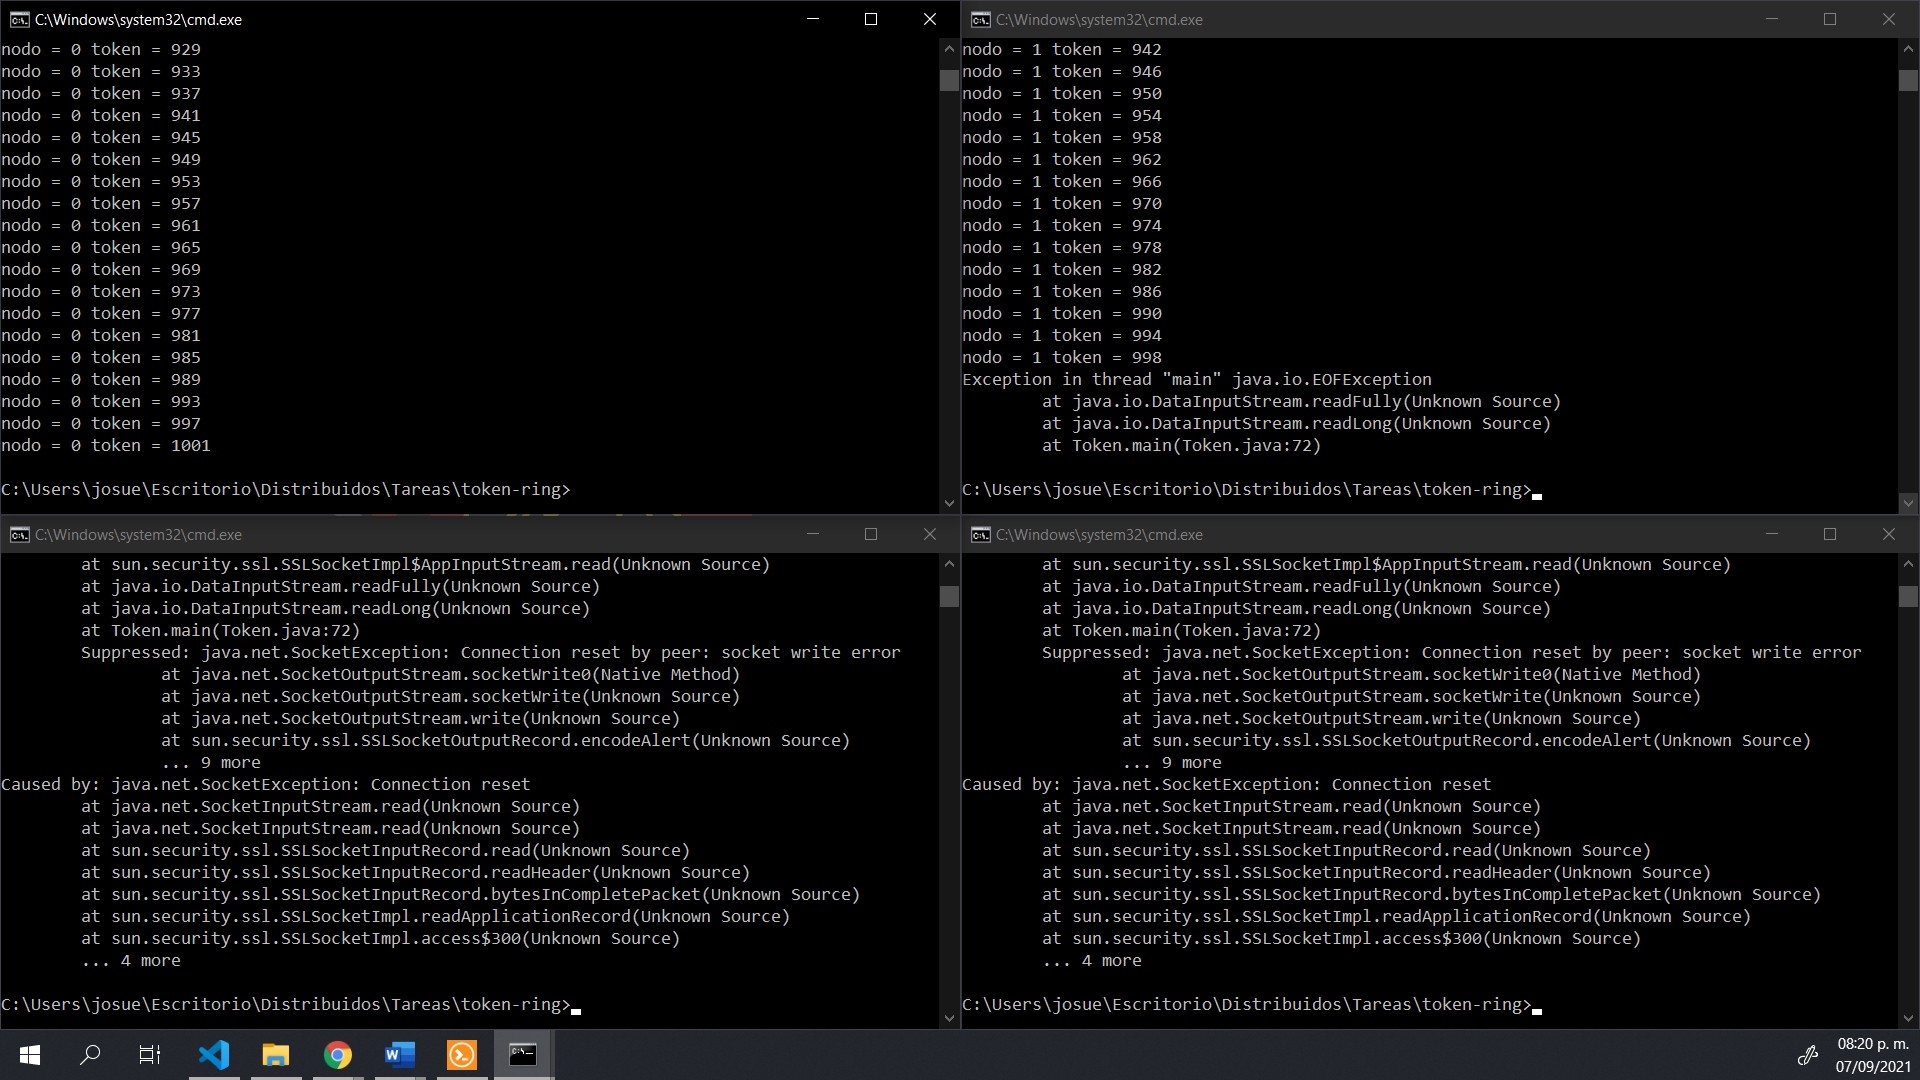
\includegraphics[scale=0.34]{resources/ejecucionfin.png}
			\caption{Consolas al final de ejecución de nuestro programa.}\label{fig:picture}
		\end{figure}
		Cuando el token se encuentre en el nodo 0 con el valor 1001 el programa terminara pero en los demás nodos se nos mostrara los errores mostrados en la figura 6, esto debido a que el nodo 0 se cierra de forma abrupta.
	\section{Conclusiones}
	El desarrollo del código de la práctica fue muy sencillo, sin embargo, añadir los sockets seguros fue algo complicado ya que en un inicio no cerraba las variables de entrada, salida y conexion algo que es sin duda alguna necesario ya que si no lo hacemos nos genera error de handshake y ese error solo se soluciona cerrando las variables anteriormente mencionadas. Mencionar que los nodos se quedaban en espera, hasta que se ejecutaran los 4 nodos totales. Los 4 nodos muestran, como salida, el numero de nodo y el valor del token, mencionar que los nodos de numero impar el valor del token mostrado en pantalla serán impares también y por otro lado los nodos pares mostraran valores de token pares. Al finalizar el nodo 0, el resto de nodos terminan de forma abrupta. \par
	Finalmente se anexan en el zip el archivo Token.java y los .jks en donde están almacenados los keystore para el cliente y el servidor.

\end{document}
